%-------------------------
%minimal-unix
%(c) H.Buchmann FHNW 2014
%export TEXINPUTS=.:${HOME}/fhnw/edu/:${HOME}/fhnw/edu/tinL/config/latex:${HOME}/fhnw/edu/config//:
%-------------------------
\documentclass{beamer}
\usepackage{latex/beamer}
%---------------------
%local defines
%(c) H.Buchmann FHNW 2009
%$Id$
%---------------------
\def \target {\raspberry\xspace}
\def \host {{\em Host \xspace}}

\input{/home/buchmann/latex/dirtree/dirtree.tex}

\usepackage[absolute]{textpos}
\setlength{\TPHorizModule}{1mm}
\setlength{\TPVertModule}{1mm}

\begin{document}

\newcommand{\md}{\cod{md-bbb-{\em version}.img}}
\newcommand{\mdev}{\cod{md-bbb-devel-{\em version}.tar.gz}}
\title[Boot]{Boot \& SD-Karten\\die verschiedenen M�glichkeiten}

\frame{\titlepage}

\section{Boot}
\begin{frame}{\target} {Die Boot Devices}
  \begin{description}
   \item[SPI0] {\bf S}erial {\bf P}eripheral {\bf I}nterface
   \item[MMC1] die eingebaute SD-Card
   \item[MMC0] die externe SD-Card
   \item[UART0] die serielle Schnittstelle
   \item[USB0] USB Schnittstelle
  \end{description}
\end{frame}

\begin{frame}{\target}{zwei M�glichkeiten}
\begin{columns}
\begin{column}{0.5\textwidth}
 \begin{itemize}
  \item die normale:
   \begin{itemize}
    \item \cod{MMC1}, \cod{MMC0}, \cod{UART0}, \cod{USB0}
   \end{itemize}
   \item Boot Switch
   \begin{itemize}
    \item \cod{SPI0}, \cod{MMC0}, \cod{USB0}, \cod{UART0}
   \end{itemize}
 \end{itemize}
\end{column}
\begin{column}{0.5\textwidth}
 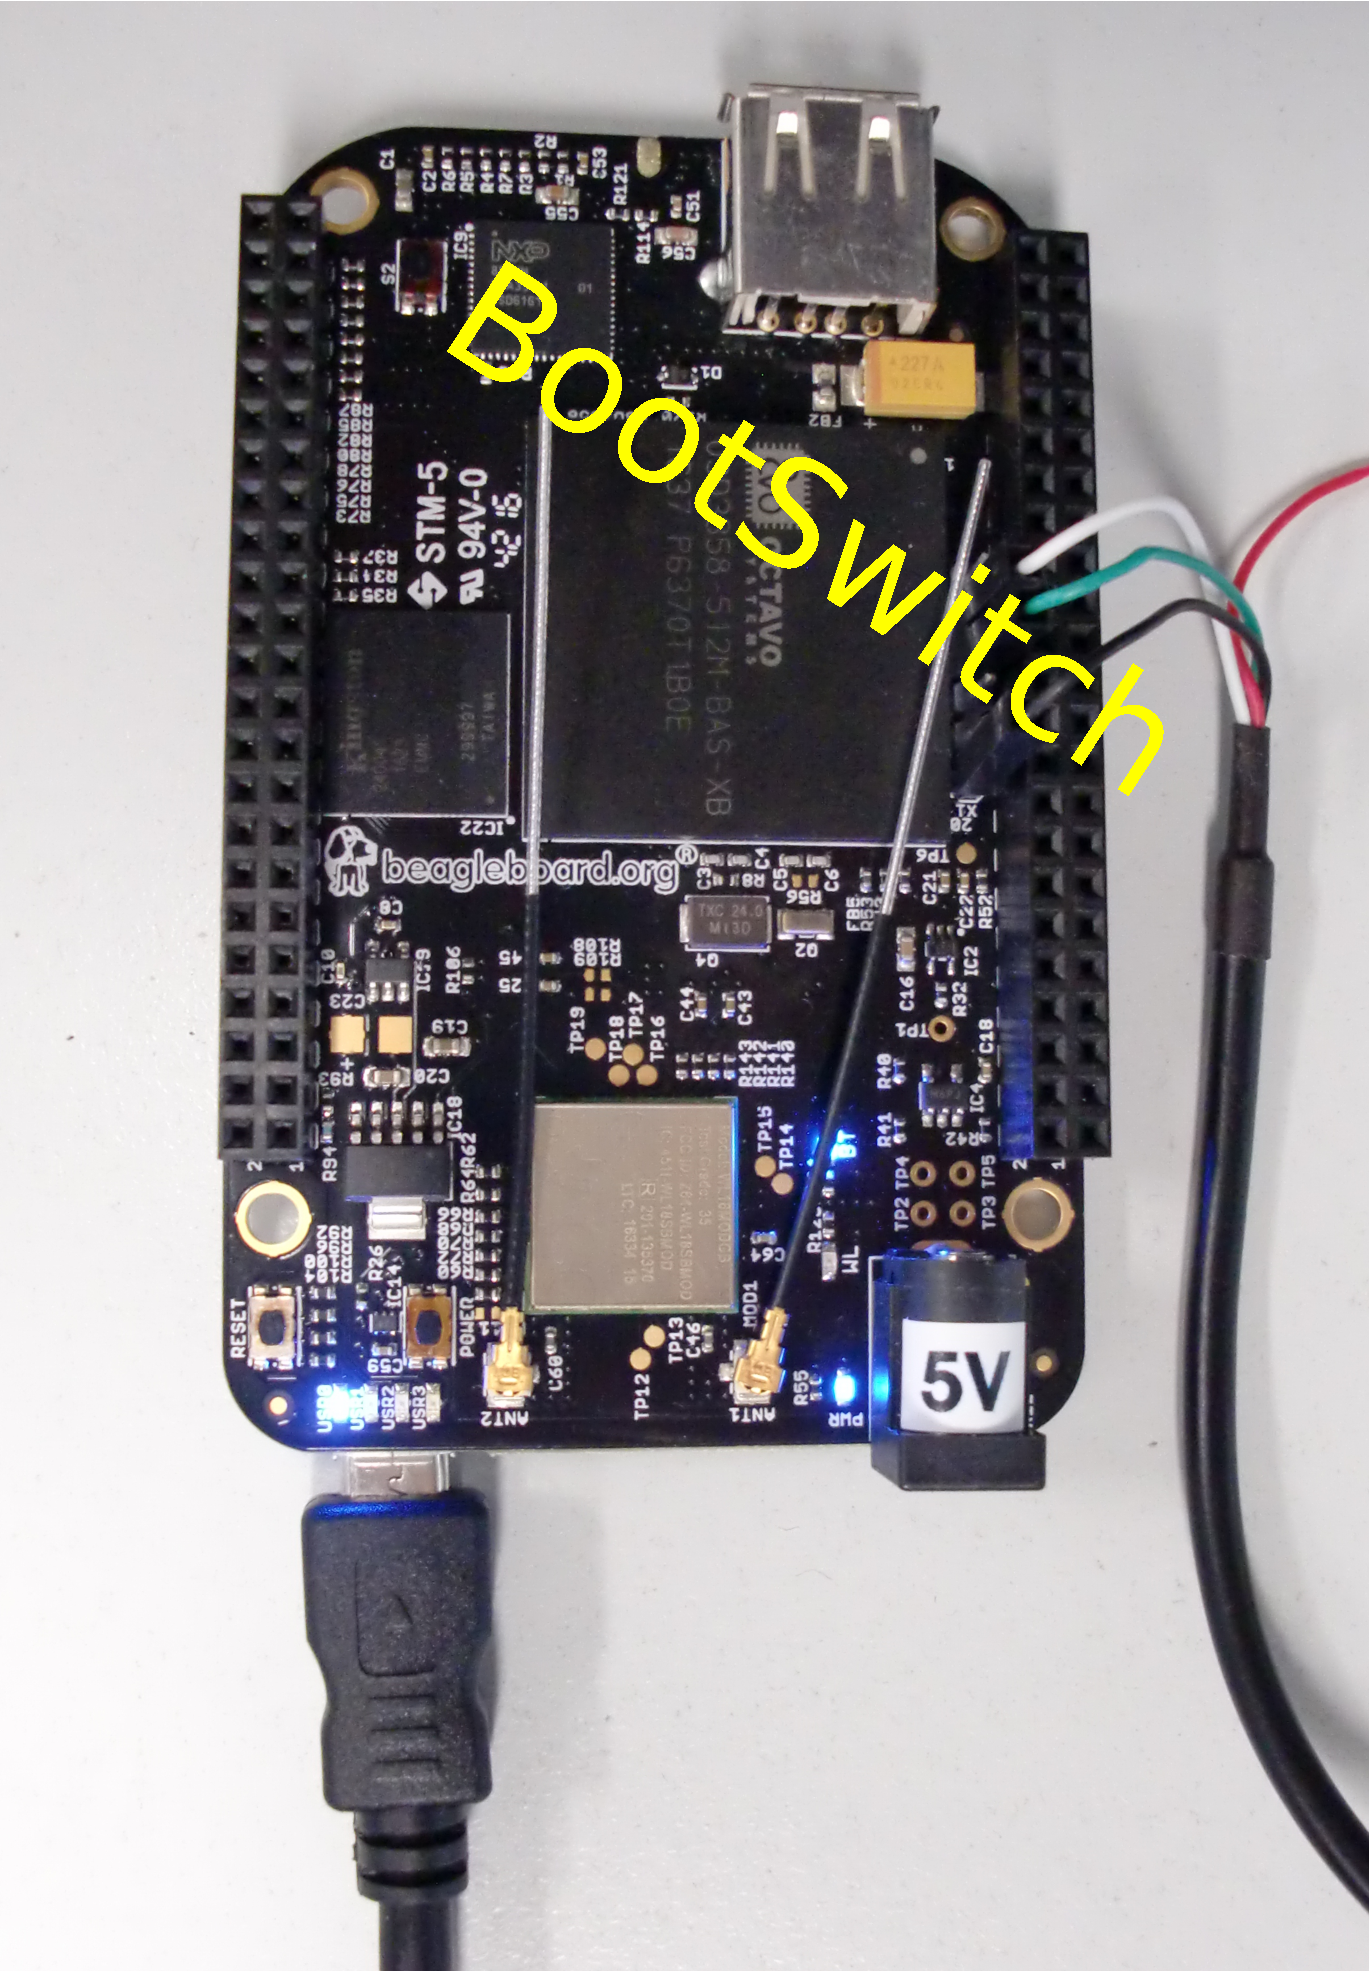
\includegraphics[width=0.75\textwidth]{bbb-boot.pdf}
\end{column}
\end{columns} 
\end{frame}

\section{SD Karte}
\begin{frame}{Initiale SD-Karte}{Herstellung}
 \begin{itemize}
  \item Daten \url{drive.switch.ch/index.php/s/wG3tEAik8mNwReA}
  \item auf SD-Karte
  \begin{itemize}
   \item \cod{sudo dd if=sd-2018-10-09.img.gz of=/dev/mmcblk0}
   \remark{{\Huge Vorsicht} bei \cod{/dev/mmcblk0}}
  \end{itemize}
 \end{itemize}
\end{frame}

\begin{frame}[fragile]{2 Partitionen}

{
\footnotesize

\begin{verbatim}
 Device         Boot Start    End Sectors  Size Id Type
/dev/mmcblk0p1 *     2048  34815   32768   16M  b W95 FAT32
/dev/mmcblk0p2      34816 559103  524288  256M 83 Linux
\end{verbatim}
}
\begin{description}
 \item[p1] Boot Partition
 \item[p2] Root Filesystem das Linux
\end{description}
\end{frame}

\end{document}
